% Created 2023-11-15 Wed 19:51
% Intended LaTeX compiler: pdflatex
\documentclass[12pt, a4paper]{article}
\usepackage[utf8]{inputenc}
\usepackage[T1]{fontenc}
\usepackage{graphicx}
\usepackage{longtable}
\usepackage{wrapfig}
\usepackage{rotating}
\usepackage[normalem]{ulem}
\usepackage{amsmath}
\usepackage{amssymb}
\usepackage{capt-of}
\usepackage{hyperref}
\usepackage{placeins}
\usepackage{gensymb}
\usepackage[letterpaper]{geometry}
\geometry{top=1.0in, bottom=1.0in, left=1.0in, right=1.0in}
\usepackage{rotating}
\usepackage{graphicx}
\usepackage{pgfplots}
\usepackage{filecontents}
\usepackage{tikz}
\usepackage{fancyhdr}
\usepackage{enumitem}
\pagestyle{fancy}
\lhead{}
\chead{}
\rhead{Johnson \thepage}
\lfoot{}
\cfoot{}
\rfoot{}
\renewcommand{\headrulewidth}{0pt}
\renewcommand{\footrulewidth}{0pt}
\setlength\headsep{0.333in}
\newcommand{\bibent}{\noindent \hangindent 40pt}
\newenvironment{workscited}{\newpage \begin{center} Works Cited \end{center}}{\newpage }
\graphicspath{ {./attachments/} }
\author{Christian}
\date{\today}
\title{}
\hypersetup{
 pdfauthor={Christian},
 pdftitle={},
 pdfkeywords={},
 pdfsubject={},
 pdfcreator={Emacs 28.2.50 (Org mode 9.7-pre)}, 
 pdflang={English}}
\begin{document}

\begin{document}
\begin{flushleft}
Christian Johnson\\
\vspace{2mm}Capt. Richard Hartnett\\
\vspace{2mm}Linear Circuits\\
\vspace{2mm}November 14 2023\\
\vspace{4mm}\begin{center}
Sallen Key Circuit Design Lab Report
\end{center}
\vspace{1mm}\setlength{\parindent}{0.5in}

\begin{abstract}
The lab focused on the practical application of the Sallen Key circuit, a fundamental element in basic filter design, to create a single second-order low-pass filter. The experiment aimed to implement real-world and simulated circuit designs, investigating the performance differences between the two. Utilizing both hardware implementation and MultiSim simulations, we explored the behavior of a second-order low-pass filter constructed from various operational amplifiers, including the LM741 and LM318. Our findings indicated a significant difference between the simulated filter and the real-world filters, forcing us to adjust our circuit design in order to adjust for the difference, and satisfy the given values. This adjustment process underscored the critical influence of real-world factors on filter performance. In the end, our exploration not only illuminated the challenges in achieving theoretical ideals but also emphasized the importance of adapting circuit designs to the intricacies of practical implementation.

\end{abstract}
\section*{Results and Analysis}
\label{sec:orgbfa0930}
In the initial phase of our experiment, we concentrated on configuring the Sallen Key circuit to achieve a desired cutoff frequency (fofo​). The following table summarizes the data obtained during this process:
\begin{center}
\begin{tabular}{lllll}
 &  &  &  & \\[0pt]
Wanted fo & 7.23 kHz & 72.3 kHz & 72.3 kHz & 72.3 kHz\\[0pt]
R Value & R = 100 kΩ & R = 10 kΩ & R = 10 kΩ & R = 9 kΩ\\[0pt]
Op-Amp & LM741 & LM741 & LM318 & LM741\\[0pt]
Degree measured & -92˚ & -90.2˚ & -89.96˚ & -90.56˚\\[0pt]
fo measured & 7.168 kHz & 55.3 kHz & 80.13 kHz & 59.65 kHz\\[0pt]
Gain (dB) & 3.67 & 13.39 & 10.8 & 13.29\\[0pt]
\end{tabular}
\end{center}

The table outlines our attempts to set the cutoff frequency at 7.23 kHz initially, subsequently changing to 72.3 kHz. For each circuit configuration, we adjusted the resistor values and utilized different operational amplifiers. The measured phase shift provides insight into the circuit's behovior, specifically, showing the circuits responsiveness to changes in frequency and resistor values. Similarly, the measured cutoff frequency deviated from intended values, indicating the real-world effect upon our components. This deviation prompted us to delve deeper into the impact of resistor selection on the circuits frequency response. Examining the gain in decibels, we observed the varying amplification levels across different configurations. These variations underscore the sensitivity of the Sallen Key circuit to component choices and influence on total gain. The results from part A help to clarify the interaction between component selection, circuit behavior, and the real-world difference from theoretical values.
Part B of our experiment focused on investigating the more specific details of the Sallen-Key circuit's behavior with different operational amplifiers and resistor configurations. We began by constructing a basic filter in Multisim, using an LM741 Op Amp, designing using resistor values to ensure that we met a design specification of f0=7.23 kHz and Q=2. This circuit is shown below, along with its magnitude and phase plot. 
\begin{figure}[htb]
\centering
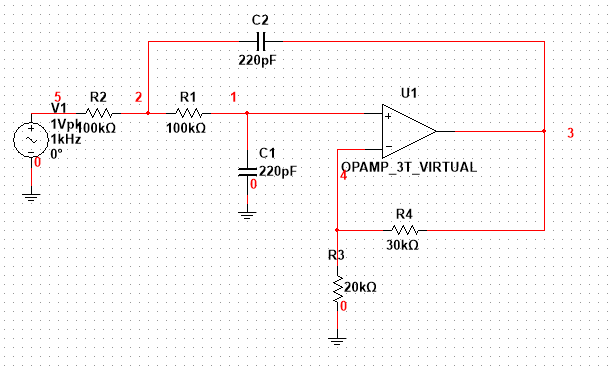
\includegraphics[width=0.7\textwidth]{Linear Sallen-Key/Multisim f7.23.png}
\caption{7.23 kHz Circuit}
\end{figure}
\begin{figure}[htb]
\centering
\includegraphics[width=0.7\textwidth]{Linear Sallen-Key/Multigraph f7.23.png}
\caption{Magnitude and Phase - 7.23 kHz}
\end{figure}
With this circuit, we were able to remain relatively close to the expected values, which this graph demonstrates. Multisim provides a realistic approximation for the circuits response. We repeated this process in order to achieve a f0 of 72.3 kHz and a Q of 2. The circuit and graphs are shown below.
\begin{figure}[htb]
\centering
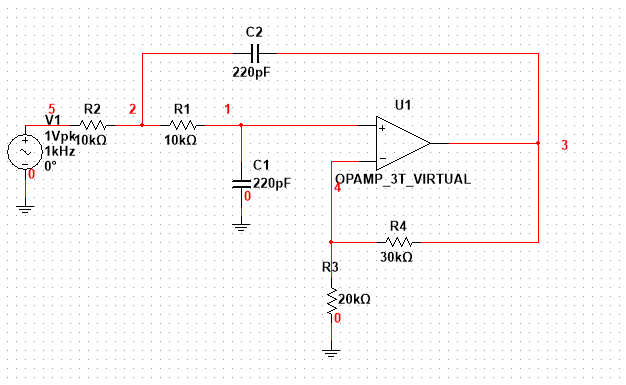
\includegraphics[width=0.5\textwidth]{Linear Sallen-Key/Multisim f72.3.png}
\caption{72.3 kHz Circuit}
\end{figure}
\begin{figure}[htb]
\centering
\includegraphics[width=0.7\textwidth]{Linear Sallen-Key/Multigraph f72.3.png}
\caption{Magnitude and Phase - 72.3 kHz}
\end{figure}
Again, we were able to achieve values that were relatively close to what we sought. 
Next, we replaces the LM741 op-amp with an LM318. We repeated our analysis from the previous step, with an f0 of 72.3 kHz and a Q of 2. Below, we see similar results to each of the previous trials.
\begin{figure}[htb]
\centering
\includegraphics[width=0.4\textwidth]{Linear Sallen-Key/Multigraph 318.png}
\caption{Magnitude and Phase plot - LM318}
\end{figure}

In Part C of this lab, we focused on taking ideal simulations that we created with Multisim and comparing those to the more realistic data from our physical circuits and Matlab. We created a physical circuit, seeking to meet the same design specifications as the simulated design we had created earlier. This physical circuit was unable to achieve these specifications with the same configuration however, due to imperfections and attenuation that does't occur in an ideal design. We were forced to compensate for this shift by changing resistors in order to satisfy the assigned design specifications. Shown below is a comparison between these three circuits, representing their phase and magnitude responses in Matlab.
\begin{figure}[htb]
\centering
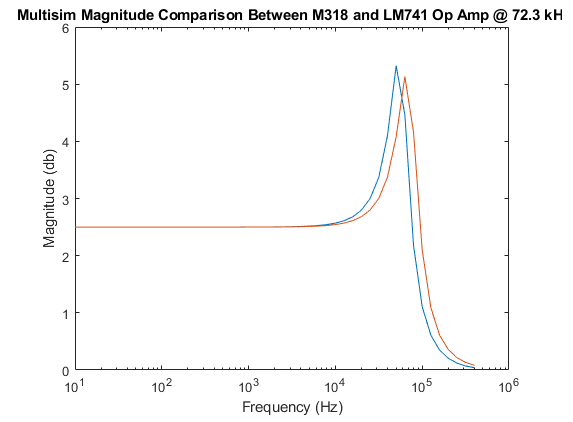
\includegraphics[width=0.45\textwidth]{MatLabGraphs/MagCompare72.3k.png}
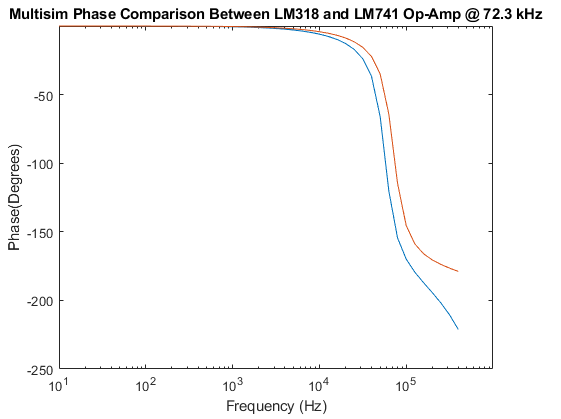
\includegraphics[width=0.45\textwidth]{MatLabGraphs/PhaseCompare72.3k.png}
\caption{Magnitude and Phase Response}
\end{figure}
For the final part of the lab, we used Matlab to overlay data from each of the trials that we had completed. We created 4 graphs from this, comparing the virtual LM741 circuit to its real world counterpart, along with theoretical predictions for ideal and real-world iterations of this circuit. We repeated this process for the LM741 at both 7.23 kHz and 72.3 kHz, and for the LM318 at the same frequencies. These graphs are shown below.
\begin{figure}[htb]
  \centering
  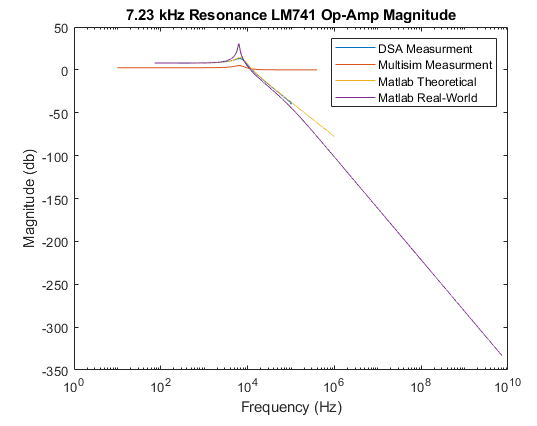
\includegraphics[width=0.45\textwidth]{MatLabGraphs/Mag7.23k.png}
  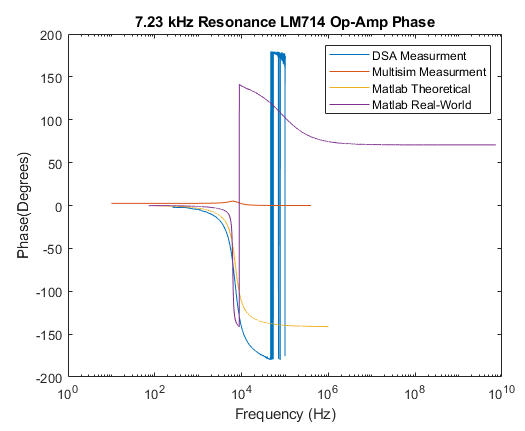
\includegraphics[width=0.45\textwidth]{MatLabGraphs/Phase7.23k.png}
  \caption{Magnitude and Phase at \(f_0 = 7.23 \text{ kHz}\)}
\end{figure}

\newpage

\begin{figure}[htb]
  \centering
  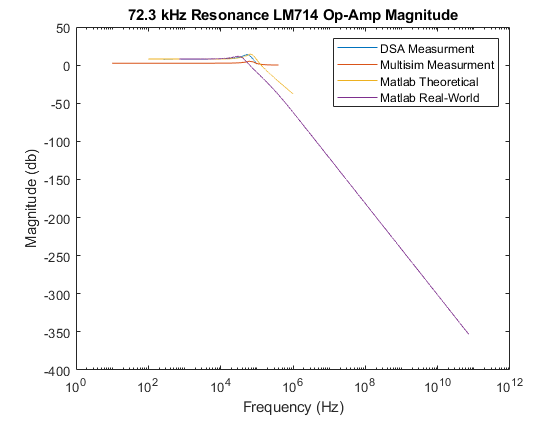
\includegraphics[width=0.30\textwidth]{MatLabGraphs/741Mag72.3k.png}
  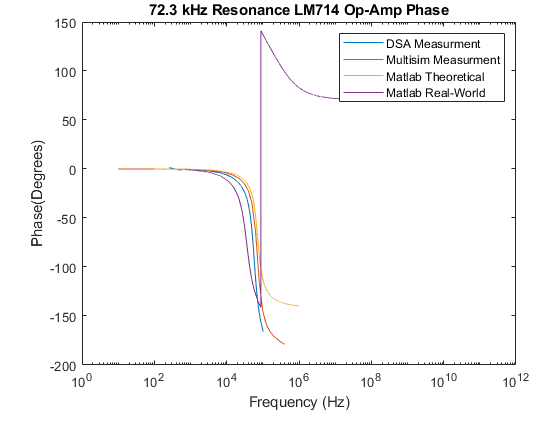
\includegraphics[width=0.30\textwidth]{MatLabGraphs/741Phase72.3k.png}
  \caption{LM741 Magnitude and Phase at \(f_0 = 72.3 \text{ kHz}\)}
\end{figure}

\begin{figure}[htb]
  \centering
  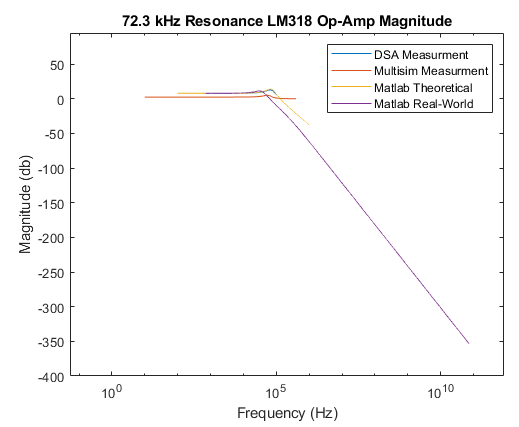
\includegraphics[width=0.30\textwidth]{MatLabGraphs/318Mag72.3k.png}
  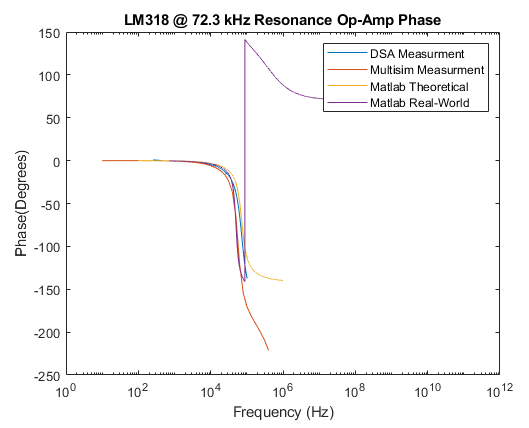
\includegraphics[width=0.30\textwidth]{MatLabGraphs/318Phase72.3k.png}
  \caption{LM318 Magnitude and Phase at \(f_0 = 72.3 \text{ kHz}\)}
\end{figure}

\begin{figure}[htb]
  \centering
  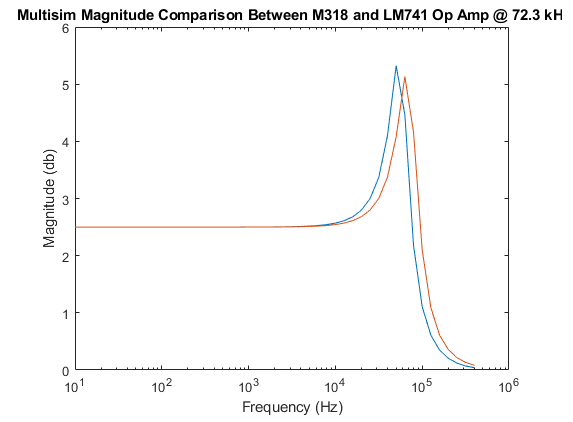
\includegraphics[width=0.30\textwidth]{MatLabGraphs/MagCompare72.3k.png}
  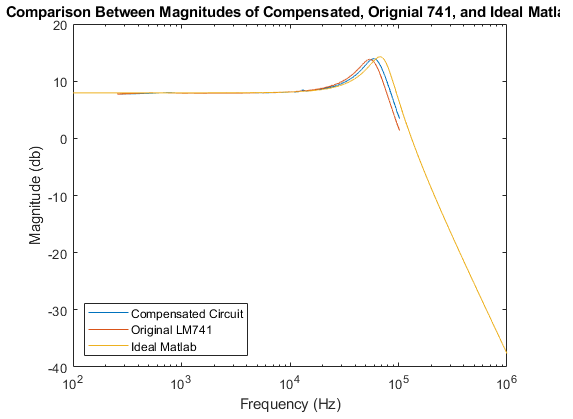
\includegraphics[width=0.30\textwidth]{MatLabGraphs/741MagComp.png}
  \caption{Magnitude Comparison and LM741 Compensated at \(f_0 = 72.3 \text{ kHz}\)}
\end{figure}
In these figures, we can see that the multisim data is relatively close to the data we received from the DSA measurement of our physical circuit. Multisim achieves a remarkeably accurate simulation of real-world response. Noteably, two of our Multisim plots did not seem to graph correctly when overlaid with the other data. These plots appear correct when shown individually, but would not work correctly in conjunction with the other graphs. 
\section*{Conclusion}
\label{sec:orgeeb0cd0}

In conclusion, this lab delved into the practical application of the Sallen Key circuit, dissecting its behavior in both simulated and real-world scenarios. We explored the circuit's response to varied component selections, which we could see in deviations in phase shift and cutoff frequencies as we sought to satisfy different specifications. The comparison between simulated results in Multisim and physical circuit responses illuminated the challenges posed by real-world imperfections. Notably, the divergence between ideal simulations and actual circuits prompted adjustments in resistor values to align with design specifications. The significance of this lies in the realization that achieving theoretical ideals requires us to adapt to the nuances of practical implementation. Furthermore, comparing different operational amplifiers, LM741 and LM318, showcased subtle differences in their performance, providing valuable insights for circuit design considerations. This comprehensive exploration underscores the importance of a nuanced understanding of circuit behavior and adaptation in bridging the gap between theoretical expectations and real-world constraints.


\end{document}
\end{document}